\documentclass[final]{beamer}

\usepackage[T1]{fontenc}
\usepackage{lmodern}
\usepackage[size=custom,width=120,height=72,scale=1.0]{beamerposter}
\usetheme{gemini}
\usecolortheme{cam}
\usepackage{graphicx}
\usepackage{booktabs}
\usepackage[numbers]{natbib}
\usepackage{tikz}
\usepackage{pgfplots}
\pgfplotsset{compat=1.14}
\usepackage{anyfontsize}

\newlength{\sepwidth}
\newlength{\colwidth}
\setlength{\sepwidth}{0.025\paperwidth}
\setlength{\colwidth}{0.3\paperwidth}

\newcommand{\separatorcolumn}{\begin{column}{\sepwidth}\end{column}}

\title{\Large The Impact of Specialized Hardware on Real-Time Processing in Embedded Systems}
\author{Group 8}
\institute[UON]{University of Newcastle, Australia}

\footercontent{
  \href{mailto:sonu.shah@uon.edu.au}{Group Members : Sonu Shah (c3507529@uon.edu.au), Rupak Pulami(rupak.pulami@uon.edu.au), Diwas Bhandari(c3508747@uon.edu.au), Sabina Paudel(c3525299@uon.edu.au), Thapa Biju(Thapa.Thapa@uon.edu.au)} \hfill
  Computing Fundamentals \hfill
  
}

\begin{document}

\addtobeamertemplate{headline}{}
{
    \begin{tikzpicture}[remember picture,overlay]
      \node [anchor=north west, inner sep=1.5cm] at ([xshift=0.0cm,yshift=1.0cm]current page.north west)
      {
\includegraphics[height=5.5cm]{logos/logo.png}}; 
    \end{tikzpicture}
}

\begin{frame}[t]
\begin{columns}[t]
\separatorcolumn

\begin{column}{\colwidth}

\begin{block}{Abstract}
   The project explores the roles played by specialized hardware (FPGAs, ASICs, GPUs) for real-time processing in embedded systems with a focus on the automotive, healthcare, and industrial automation sectors. It also teaches integrated programming, which uses integrated hardware and software to increase speed, efficiency, and reliability. This work compares general-purpose and specialized hardware, addresses related challenges and trade-offs, and analyses performance and practical implications of hardware specialization in embedded systems though case studies.
  \end{block}



  \begin{block}{Introduction}
    Embedded systems are tailored computing systems that perform dedicated functions. In real-time applications like automotive systems, medical devices, and robotics, the ability to process data immediately is critical. This project explores how specialized hardware such as FPGAs, ASICs, and GPUs enhance real-time processing capabilities in embedded systems.
  \end{block}

  \begin{block}{The Need for Real-Time Processing}
   Analogous to microcontrollers, embedded systems are specialized computer systems that handle dedicated functions within a larger mechanical or electrical system. These systems are dedicated to a specific set of tasks and general-purpose computing systems are however optimized and they operate with limited pure hardware. Many embedded systems demand real-time event handling, with responses delivered within strict time limits. In fundamental systems, such as automotive safety or industrial automation, missing these deadlines may have catastrophic implications. Real-time systems can be hard (where a missed deadline is unacceptable) or soft (where delays degrade performance but are tolerable).
  \end{block}
  
 \begin{alertblock}{Key Hardware Technologies}
    \begin{itemize}
      \item \textbf{FPGAs (Field Programmable Gate Arrays):} Reconfigurable logic ideal for custom data paths and parallelism.
      \item \textbf{ASICs (Application Specific Integrated Circuits):} Highly efficient for specific tasks, with minimal latency.
      \item \textbf{GPUs (Graphics Processing Units):} Excellent for tasks involving matrix operations and parallel computation.
    \end{itemize}
  \end{alertblock}
  
   \begin{block}{Comparative Analysis of Hardware Solutions}
   Comparative research is employed to evaluate the usability of FPGAs, ASICs, and GPUs in real-time embedded systems. These hardware types are analyzed across five key parameters:
   \begin{itemize}
       \item Performance: Efficiency in executing real-time tasks.
       \item Power Efficiency: Power consumption relative to computational workload.
       \item Flexibility: Programmability and adaptability for diverse tasks or configurations.
       \item Cost & Development Time: Trade-off between initial cost, manufacturing expenses, and ease of design.
       \item Scalability: Suitability for diverse applications and readiness for mass production.
   \end{itemize}
  \end{block}

 

\end{column}

\separatorcolumn

\begin{column}{\colwidth}

  \begin{block}{Performance Comparison}
    \begin{itemize}
      \item FPGAs and ASICs outperform general CPUs in terms of real-time responsiveness.
      \item GPUs offer massive parallelism but may introduce latency in communication overhead.
      \item Performance metrics: latency, throughput, energy efficiency.
    \end{itemize}
  \end{block}

  \begin{block}{Case Study: Autonomous Vehicles}
    Real-time object detection and decision-making are critical.
    \begin{itemize}
      \item FPGAs used for sensor fusion.
      \item GPUs process computer vision and deep learning models.
      \item ASICs control braking and steering systems.
    \end{itemize}

    \begin{figure}[H]
  \centering
  \begin{tikzpicture}
    \node[anchor=center] at (0,0) {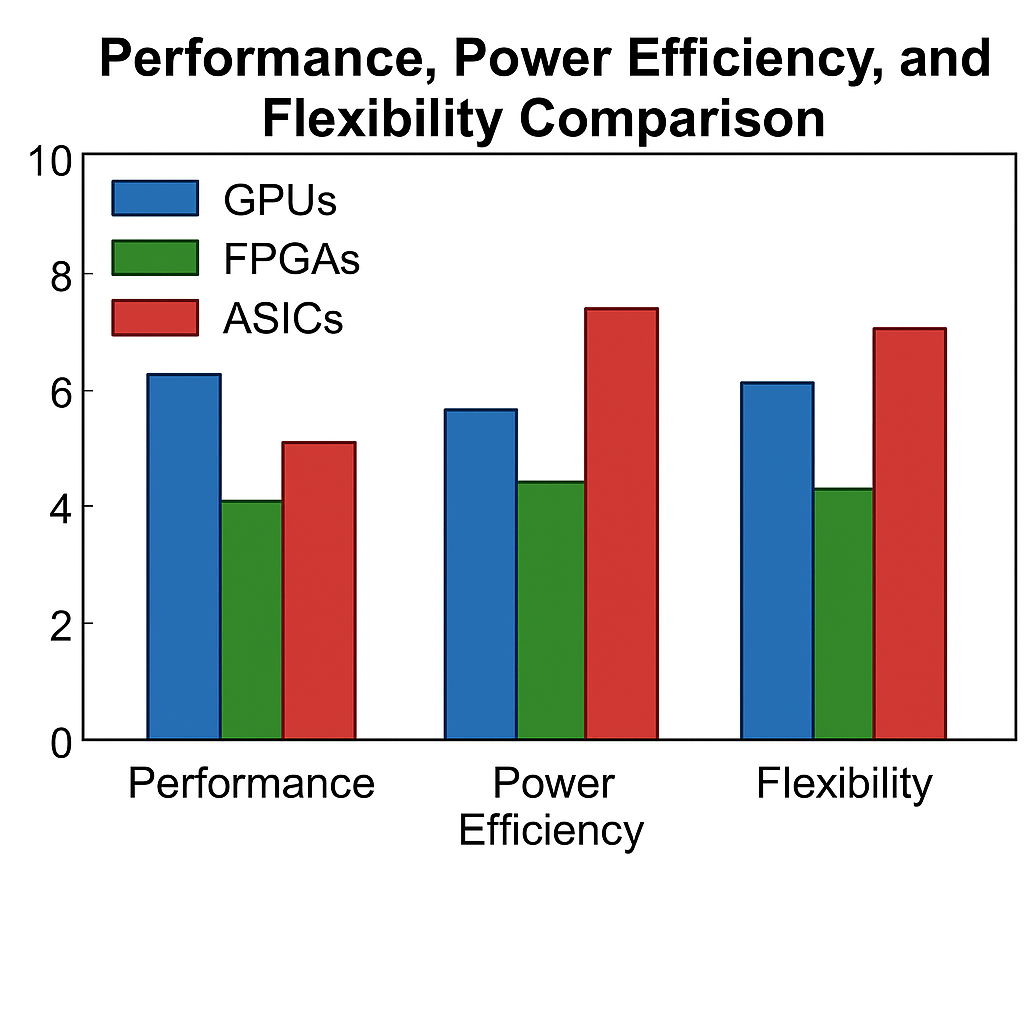
\includegraphics[width=0.7\linewidth]{logos/Performance, efficiency and flexibility comparsion.png}};
  \end{tikzpicture}
  \caption{Performance, Efficiency, and Flexibility Comparison of Specialized Hardware}
\end{figure}
  \end{block}

  \begin{block}{Challenges}
    \begin{itemize}
      \item \textbf{Cost and complexity} of specialized hardware.
      \item \textbf{Power consumption} in high-performance devices.
      \item \textbf{Integration difficulty} with legacy systems.
    \end{itemize}
  \end{block}

\end{column}

\separatorcolumn

\begin{column}{\colwidth}

  \begin{exampleblock}{Conclusion}
    Using specialized hardware, such as GPUs, FPGAs, and ASICs, in real-time embedded systems can
result in a huge performance boost by improving speed, lowering latency, and optimizing the power
consumption. GPUs shine for tasks that run in parallel, while FPGAs allow for great flexibility and
ASICs deliver impressive efficiency for particular functions.
There are trade-offs in cost and scalability, but integrated programming can helpwith bridging hard-
ware and software for reliable, time-sensitive processing. As embedded technology continues to advance,
hybrid systems that incorporate these types of hardware will playa crucial role in shaping the future of
embedded solutions
  \end{exampleblock}

  \begin{block}{Future Scope}
    \begin{itemize}
      \item Artificial Intelligence integration for literary smarter and adaptive embedded systems.
      
      \item High performance, ultra low-power ASIC design for wearable and medical system solutions.
      
      \item development and deployment of FPGA tools.
      
      \item Real-time decision-making at the source through edge computing.
      
      \item High-performance CPU-GPU-FPGA SoC architecture
      
    \end{itemize}
  \end{block}

  \begin{block}{References}
1. Liu, J. W. S. (2000). Real-Time Systems. Prentice Hall.

2. Wolf, W. (2001). Computers as Components: Principles of Embedded Computing System Design.
Morgan Kaufmann.

3. Marwedel, P. (2010). Embedded System Design: Embedded Systems Foundations of Cyber-
Physical Systems. Springer.

4. Mittal, S. (2016). “A Survey of Techniques for Improving Energy Efficiency in Embedded Com-
puting Systems.” International Journal of Computer Aided Engineering and Technology, 8(6), 721–741.

5. Zhang, Y., Zhao, J. (2019). “FPGA-Based Acceleration Techniques for Deep Learning Applica-
tions: A Survey.” ACM Transactions on Reconfigurable Technology and Systems, 12(3), 1-26.

6. Chen, Y., Emer, J., Sze, V. (2016). “Eyeriss: A Spatial Architecture for Energy-Efficient Dataflow
for Convolutional Neural Networks.” ACM SIGARCH Computer Architecture News, 44(3), 367-379.

    \footnotesize
    \bibliographystyle{plainnat}
    \bibliography{poster}
  \end{block}

\end{column}

\separatorcolumn
\end{columns}
\end{frame}

\end{document}